\documentclass[11pt,a4paper]{article}
\usepackage[T1]{fontenc}
\usepackage[ngerman]{babel}
\usepackage{amsmath}
\usepackage{parskip}
\usepackage{graphicx}
%\usepackage{listings}
\usepackage{hyperref}
\usepackage{float}

%opening
\author{Simon Cholewa}
\title{11. Decision Trees Exercise}

\hyphenation{
	Mo-tor-ü-ber-wach-ung 
}


\begin{document}

\maketitle

\section{}

\textit{Find some data here \hyperref{https://drive.google.com/open?id=1E3bFrHnMGGmBgyAk9vAVnHGpQ8Z_asOP}{}{}{[1]} on people. The goal is to decide if someone buys a computer or not. Derive the best decision tree by calculating a little by hand (Shannon). At least the first split. }

\begin{figure}[h!]
	\centering
	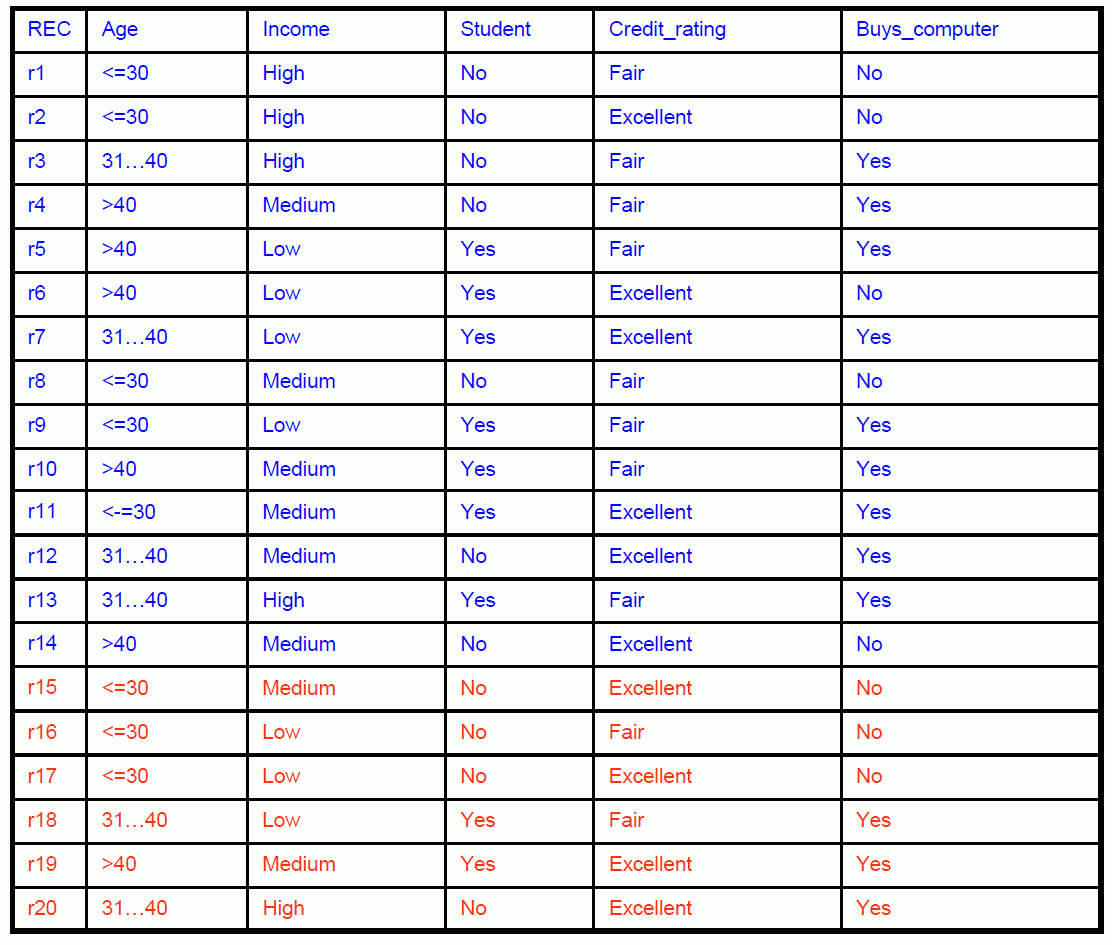
\includegraphics[width=1\linewidth]{DATA}
	\caption{Daten aus [1], mit denen der Decision Tree erstellt werden soll.}
	\label{fig:data}
\end{figure}


\subsection*{Step 1}

\textit{Calculate entropy of the target.}

Die Entropie der Spalte \textit{Buys\_computer} ist 0.971.

\subsection*{Step 2}

\textit{The dataset is then split on the different attributes. The entropy for each branch is calculated. Then it is added proportionally, to get total entropy for the split. The resulting entropy is subtracted from the entropy before the split. The result is the Information Gain, or decrease in entropy.}


age <=30:  0.8112781244591328\\
age 31..40:  0.0\\
age >40:  0.9182958340544894\\
Entropy of property age: 0.6\\
Information gain when using age:  0.371

income High:  0.9709505944546688\\
income Medium:  0.954434002924965\\
income Low:  0.9852281360342515\\
Entropy of property income: 0.97\\
Information gain when using income:  0.002

student False:  0.9456603046006401\\
student True:  0.5032583347756457\\
Entropy of property student: 0.75\\
Information gain when using student:  0.224

credit\_rating Fair:  0.8812908992306927\\
credit\_rating Excellent:  1.0\\
Entropy of property credit\_rating: 0.94\\
Information gain when using credit\_rating:  0.03

information\_gain\\
age                    0.370951\\
student                0.224371\\
credit\_rating          0.030305\\
income                 0.001609\\


\subsection*{Step 3}
\textit{Step 3: Choose attribute with the largest information gain as the decision node, divide the dataset by its branches and repeat the same process on every branch.}

The highest information gain is provided by AGE.


\subsection*{Step 4a}
\textit{A branch with entropy of 0 is a leaf node.}

AGE 31..40 is a leaf.

\subsection*{Step 4b}
\textit{Branch with entropy more than 0 needs further splitting.}

AGE <=30 is not a leaf.
AGE >40 is not a leaf.

Abbildung \ref{fig:graphlevel1} zeigt eine Darstellung des Zwischenergebnisses.

\begin{figure}
	\centering
	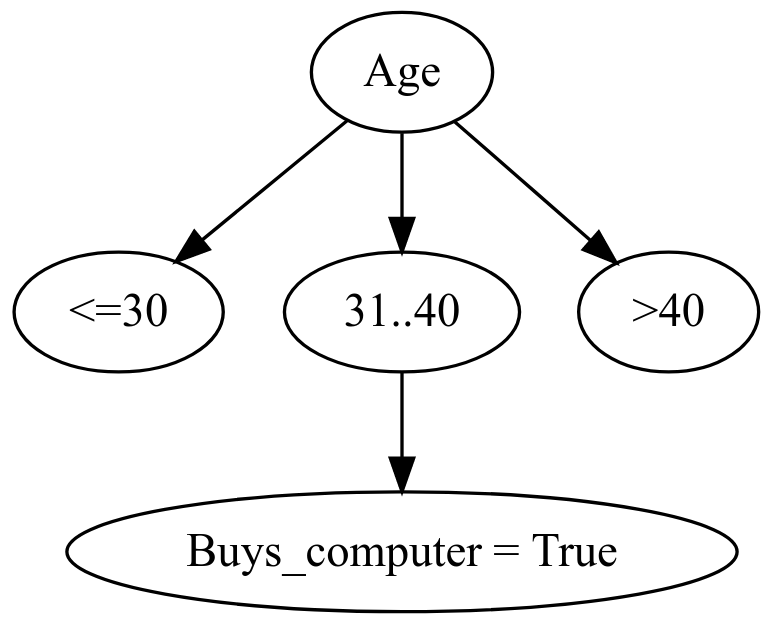
\includegraphics[width=0.5\linewidth]{bilder/graph_level1}
	\caption{Der Entscheidungsbaum nach dem ersten Split}
	\label{fig:graphlevel1}
\end{figure}


\subsection*{Wiederholung der Schritte 1-4}

Vom Knoten \textit{<=30} bringt den größten Informationsgewinn der Parameter \textit{student} (0.971 Bit). In dieser Altersgruppe kaufen nur Studenten Computer. Somit entstehen zwei Blätter.

Vom Knoten \textit{>40} bringt den größten Informationsgewinn der Parameter \textit{credit\_rating} (0.833 Bit). Ist das \textit{credit\_rating} in dieser Altersgruppe \textit{Fair}, wird ein Computer gekauft. Es liegt hier ein weiteres Blatt vor.

Im nächsten Schritt (\textit{credit\_rating = Excellent}) liefern die Fragen nach Status als Student oder Einkommen den gleichen Informationsgewinn. Ich entscheide mich für \textit{income}. Somit folgt hier als letztes Kriterium \textit{student}. Der so erstellte Entscheidungsbaum wird in Abbildung \ref{fig:graphcomplete} dargestellt.

\begin{figure}
	\centering
	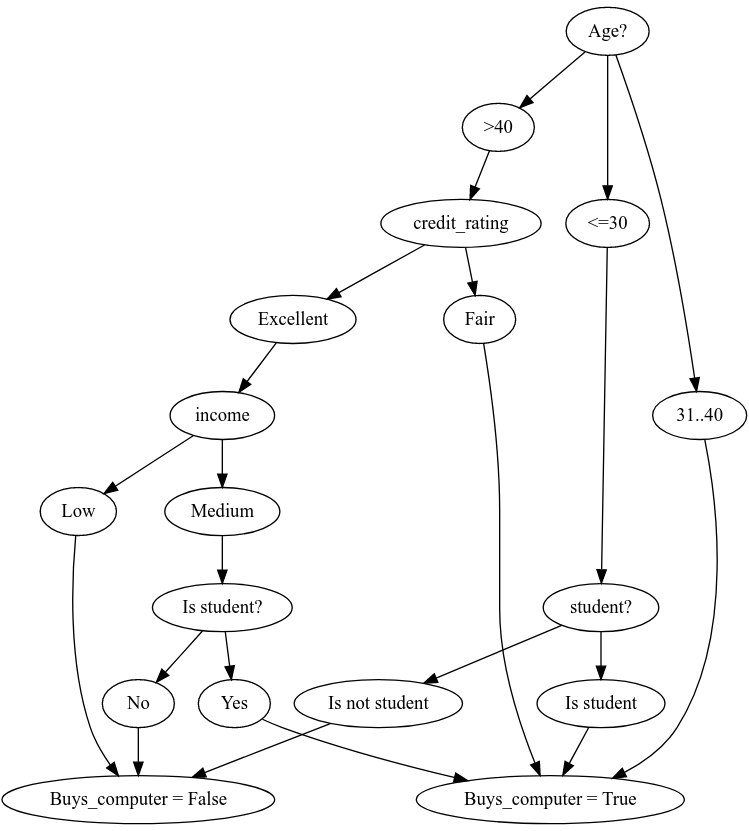
\includegraphics[width=0.9\linewidth]{bilder/graph_complete}
	\caption{Der vollständige Entscheidungsbaum.}
	\label{fig:graphcomplete}
\end{figure}


\section{}

\textit{Compare your tree against the tree derived from SciKit Learn as given in the Python example before! Why are they different? Print the tree with Graphviz (can be easily done with \hyperref{http://www.webgraphviz.com/}{category}{name}{WebGraphViz [2]})}

Siehe Abbildung \ref{fig:treescikitentropy} für die Darstellung. Die Kategorien mussten als Zahlen dargestellt werden:

\texttt{X = X.replace('<=30', 30).replace('31..40', 35).replace('>40', 41)
X = X.replace('High', 10).replace('Medium', 5).replace('Low', 0)
X = X.replace('Excellent', 10).replace('Medium', 5).replace('Fair', 0)}

Weil hier nicht mit Nominal- oder Ordinalkategorien gearbeitet wurde (Ausnahme: Boolsche-Kategorien), wurden die verwendeten Platzhalter zum Rechnen verwendet. Ich habe für die Altersklassen die Zahlen 30, 35 und 41 gewählt. Daraus wurde die Abfrage $age \leq 32.5$. Es kann hier immer nur zwischen zwei Klassen gewählt werden.

\begin{figure}
	\centering
	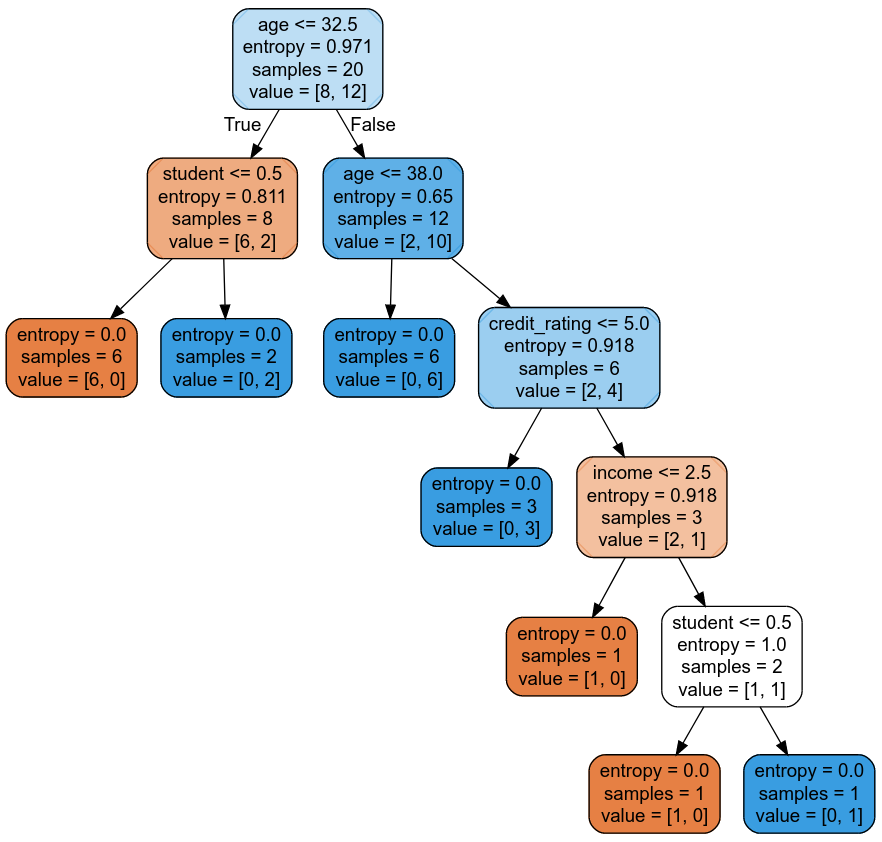
\includegraphics[width=1\linewidth]{bilder/tree_scikit_entropy}
	\caption{Der vollständige von SciKit Learn berechnete Entscheidungsbaum.}
	\label{fig:treescikitentropy}
\end{figure}

\end{document}
